\section{Wirtualizacja i orkiestracja}
% myślę, że opisanie tego jak wirtualizacja pomaga w CI/CD zasługuje na swój rozdział.
% Szczególnie mógłbym ten rozdział poświęcić dockerowi z faktu, że zdominował rynek.
% Warto tutaj byłoby napisać też o rozwiązaniach które były używane w przeszłości a zostały wyparte jak vagrant.
% Dodatkowo w rozdziale mozemy opisać na czym polega orkiestracja - Kubernates, docker swarm

\subsection{Wirtualizacja - początki}
Opisując automatyzację w procesów w przemyśle IT konieczne jest opisać wirtualizacje czyli kojelny kamień milowy w budowanie intrastruktury oraz współczesny sposob wytwarzania i dostarczania oprogramowania. Czym tak właściwie jest wirtualizacja? 
Żeby dobrze zrozumieć jak istotną role odgrywa wirtualizacja w automatyzacji warto spojrzeć wstecz i przyjrzeć się historii serverów i komputerów wogóle.   Jak podaje Paul E. Ceruzzi czyli autor książki "A History of Modern Computing", w przeszłości jeśli była potrzeba uruchomienia serwera, były zasadniczo dwie opcje: 
\begin{itemize}
    \item zbudować swój własny fizyczny serwer
    \item wynająć/kupić sprzęt komputerowy od firmy, która takie usługi prowadzi
\end{itemize}
W pierwszym przypaku budowanie własnego serwera wymaga duzej liczby inżynierów z odpowiednią wiedzą i doświadczeniem, narzędzi oraz materiałów do budowy. Niekażda firma będzie więc spełnić te wszystkie wymagania dlatego drugą opcją stała się więc zdecydowanie bardziej popularna. Pierwszą firmą która skorzystała na trudzie wykonania własnego serwera była firma IBM i tak w 1960 powstał IBM Mainframe, czyli sprzęt najwyższej klasy jak na uwczesne możliwości.

\begin{figure}[htbp]
    \centering
    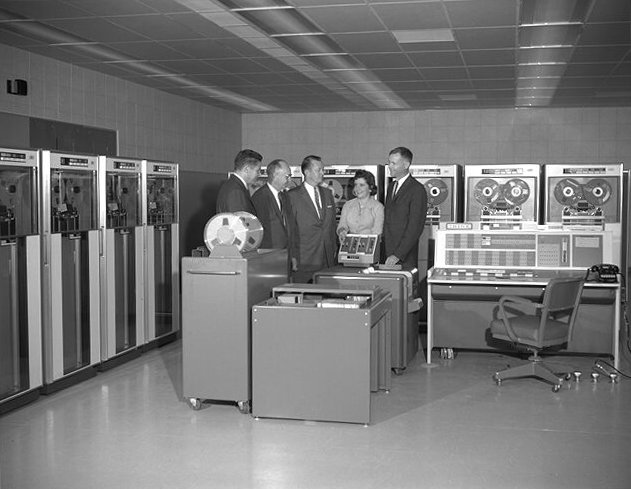
\includegraphics[width=10cm]{IBM-computer.jpg}
    \caption{IBM Mainframe}
    \label{fig:ibm-mainframe}
\end{figure}

Przez kolejne 20 lat sprzęty komupterowe firmy IBM dominowały rynek. Początkowo na Mainframie mozna było uruchomić tylko jedną aplikację do powodowało duze marnotratwo zasobów i czasu. Później została dodana wielozadaniowość co znacznie usprawniło działanie sprzętu. W 1980 roku był wielki "boom" technologiczny, który testował mozliwości serwera. Szybko się okazało, ze utrzymanie serwerów jest kosztowne. Konserwacja sprzetu, miejsce w którym serwery są przechowywane oraz koszty związane z administrowaniem sprawiły, ze na rynku pojawiła się potrzeba na technologie wirtualizacyjne i tak w latach 90 XX wieku w połączenie wydajnych procesów oraz znawców z dziedziny sprzętu komputerowego powstału wirtualne maszyny i wirtualizacja wogóle. 

\subsection{Czym są wirtualne maszyny?}
Wirtualne maszyny są kolejną warstwą abstrakci między urzytkownikiem a "metalem", czyli fizyczym sprzętem. Dzięki wykorzystnaiu tego mechanizmu, zamiast jednego systemu operacyjnego uruchomionego na komputerze, mozliwe jest uruchomienie wielu "gości" systemu operacyjnego na bazowym systemie operacyjnym. Dlaczego to jest takie przydatne? Teraz posiadając jedną mocną maszynę mozemy dowolnie dodawać i usuwać serwery. Tak wiec jeśli  teraz dodam dodatkową funkcjonalność do mojego programu, jedyne co muszę zrobić zeby go wdrozyć jest dodanie dodatkowej virtualnej maszyny jednym z serwerów, który ma wystarczająco duzo miejsca, żeby to zrobić. To rozwiązanie daje bardzo dużo elastycznosci. 
Jak dokładnie działa zarządzanie zasobami na wirtualnej maszynie?
Mechanizm dzięki któremu jest możliwa wirtualizacja nazywa się hypervisor. Hypervisor zarządza całym cyklem życia oraz funkcjonalnością wirtualnej maszyny. 
Do jego głównych zadań należą:
\begin{itemize}
    \item alokacja odpowiedinej ilości RAM'u, mocy obliczeniowej, pamięci dyskowej oraz zarządanie połączeniem z siecią
    \item startowanie wirtualnej maszyny 
    \item czyszczenie zasobów po zatrzymaniu wirtualnej maszyny
    \item zapewnianie izolacji dla odzielnie działających wirtualnych maszym 
    \item zarządzanie wirtualnymi maszynami
\end{itemize}
oraz wiele innych. 
Tak wiec podsumowując, jest jeden bazowy system operacyjny uruchomiony na komputerze, który udostępnia zasoby serwera wirtualnym maszynom i jeśli zasoby na tej wirtualnej maszynie się wyczerpią to nie ma to żadnego wpływu na inne wirtualne maszyny uruchomione na tym serwerze. Dodawtkowo pliki między wirtualnymi maszynami nie są współdzielone co sprawia, ze jeśli na jednej z wirtualnych maszyn zostanie usuchomiony niebezpieczny skrypt, szkody wyrządzone zostaną ograniczone do jednego systemu co sprawia, ze jest to rozwiązanie relatywnie bezpiecznie.
Wszystkie powyższe zalety nie są jednak "za darmo". Uruchamianie systemu operacyjnego wewnątrz innego systemu nie jest optymane jeśli chodzi o wydajność natomiast korzyści jakie niesie ze sobą wirtualizacja sprawiają, że jest ona wykorzystywana do dzisiaj w środowiach przemysłowych jak i naukowych. 
\subsection{Chmura publiczna}
W raz z rozwojem technologii rozwijali sie dostawcy chmury obliczeniowej tacy jak Microsoft Azure czy Amazon Web Services, u których mozna wynająć wirtualną maszynę. Maszyna ta będzie wyposazona w wstepnie przydzielona pamięcią ram oraz moca obliczeniowa (często moc obliczeniową nazywane są vitual cores bądź vCores). 
Zaletą tego podejścia jest brak konieczności utrzymywania serwerowni ale wciąż osoby wynajmujące odpowiedzialne są za utrzymanie oprogramowania które jest uruchamiane na serwerach. 
Dzięki chumurom możemy dynamicznie skalować nasze wirtualne maszyny, jedynym ograniczeniem są koszty jakie jesteśmy w stanie ponieść. Dostawaca jedynie dostarcza wirtualne maszyny, natomiast koniecznym wciąż jest zarządzanie całym oprogramowaniem, siecią, zaopatrzeniem, aktualizacją, itp. Wiele firm wciąż wybiera to rozwiązanie dlatgo powstały narzędzia jak Terraform, Chef, Puppet, Salt oraz wiele innych by ten proces maksymalnie uprościć. 
Podejściem tym jednak wciąż zgadzamy się na konsekwencje jakie niesie ze sobą uruchamianie jednego wystemu operacyjnego w drugim. Czy nie było by super gdybyśmy mogli wykorzystać system operacyjny hosta bez obawy, że marnujemy tak cenne zasoby naszego komputera? To właśnie było motywacją do powstania kontynerów czyli sposobu na budowanie infrastruktury dziś. 
\subsection{Kontynery}
Jak pewnie można sobie wyobrazić, kontynery dają nam wiele korzyści które niesie ze sobą wirtualna maszyna takie jak bezpieczeństwo oraz zarządzanie zasobami ale bez marnowania zasobów na system operacyjny. W kontynerach system operacyjny jest zastąpiony trzeba możliwościami jakie daje linux: chroot, namespace oraz cgroup by oddzielić między sobą wrażliwe komponenty na naszej maszynie.
Żeby dobrze rozumieć czym jest kontyner oraz jak dużym krokiem na przód są dzisiejsze narzędzia do tworzenia kontynerów, w daleszej części pracy stworzę kontyner "ręcznie" wykorzystując wyżej wymienione filary kontynera. Wykonywane komendy będą uruchamiane na Ubuntu 18.04.3 LTS

\subsection{Chroot}
To jest linuksowa komenda, która pozwala zmienić bazowy katalog dla nowego processu. W tym ćwiczeniu ustawię bazowy katolog w wcześniej utworzony katalog co rozwiążemy problem bezpieczeństwa ponieważ processy na naszym kontynerze nie będą "widoczne" poza katalog bazowy. 
Aby zmienić katalog bazowy, stwórzmy wpierw nowy folder który będzie pełnił taką role "mkdir /my-new-root". Następnie przekopujmy podstawowe programy dostępne w systemie linux. "cp /bin/bash /bin/ls /my-new-root/bin/" oraz teraz musimy przekopiować biblioteki wykorzystując następujące kroki
\begin{lstlisting}
    - mkdir /my-new-root/lib{,64}
    - cp /lib/x86_64-linux-gnu/libtinfo.so.5 /lib/x86_64-linux-gnu/libdl.so.2 /lib/x86_64-linux-gnu/libc.so.6 /my-new-root/lib
    - cp /lib64/ld-linux-x86-64.so.2 /my-new-root/lib64
    - cp /lib/x86_64-linux-gnu/libselinux.so.1 /lib/x86_64-linux-gnu/libpcre.so.3 /lib/x86_64-linux-gnu/libpthread.so.0 /my-new-root/lib
\end{lstlisting}
Jeśli te kroki poprawnie wykonamy powinniśmy być wstanie urzyć komendy chroot /my-new-root bash oraz ls. W ten właśnie sposów zmieniamy katalog bazowy. 
\subsection{Namespaces}
Dzięki chroot sprawiliśmy, że dostęp do plików hosta z nowego kontynera będzie niemożliwy ale wciąż możemy ubić proces, zniszczyć system plików bądź nawet przechwytywać processy. 
Dzięki namespacom mamy możliwość "chowania" processów przed innymi processami. 
Zróbmy więc nasz nowy kontyner bardziej bezpiecznym. W tym celu posłużymy się komendą 'unshare', która uwtorzy nowy wyizolowany namespace z manespacu rodzica.

\begin{lstlisting}
    # instalowanie bootstarapa
    apt-get update -y
    apt-get install debootstrap -y
    debootstrap --variant=minbase bionic /better-root

    # zmiana namespace'a
    unshare --mount --uts --ipc --net --pid --fork --user --map-root-user chroot /better-root bash # this also chroot's for us
    mount -t proc none /proc # process namespace
    mount -t sysfs none /sys # filesystem
    mount -t tmpfs none /tmp # filesystem
\end{lstlisting}
powyższe komendy utorzą nowe środowisko z odizolowanymi processami, dyskami oraz siecią. Teraz nasz nowy kontyner juz nie widzi żadnych processów!
\subsection{cgroups}
W tym momencie mamy zabezmieczenie przed bałagnem w strukturze plików, processy się zgadzają ale co z zasobami? czy nie będzie tak, że jeśli wyczermie się załóżmy pamieć na jednym kontynerze to wszystkie inne przestaną działać? Na ten moment tak właśnie będzie i tu z pomocą przychodzą nam kontrol grupy (cgroups). Mechanizm ten polega na przydzielaniu zasobów hosta do jego dzieci na zasadzie jesli przekroczysz limit to koniec więcej nie będzie. 

Tutaj w jaki sposów wykorzystałem cgrupy w naszym kontynerze: 

\begin{lstlisting}
    apt-get install -y cgroup-tools htop
    cgcreate -g cpu,memory,blkio,devices,freezer:/sandbox
    ps aux 
    cgclassify -g cpu,memory,blkio,devices,freezer:sandbox <PID>

    cat /sys/fs/cgroup/cpu/sandbox/tasks
    cat /sys/fs/cgroup/cpu/sandbox/cpu.shares

    cgset -r cpu.cfs_period_us=100000 -r cpu.cfs_quota_us=$[ 5000 * $(getconf _NPROCESSORS_ONLN) ] sandbox

    cgset -r memory.limit_in_bytes=80M sandbox
    cgget -r memory.stat sandbox

    htop # will allow us to see resources being used with a nice visualizer

    yes > /dev/null # this will instantly consume one core's worth of CPU power
    yes | tr \\n x | head -c 1048576000 | grep n # this will ramp up to consume ~1GB of RAM
\end{lstlisting}
na ten moment mamy stworzony kontyner w najprostrzej postaci a pomimo, że nie poruszyliśmy niezwykle istotynych aspektów jak networking, deploying i building. 
Jak można zauważyć pisanie wszystkiego ręcznie nie jest trywialnym zadaniem. Dlatego na rynku pojawiłi się rozwiązania jak Docker do tworzenia, aktualizacji, zarządzania uruchomionymi kontynerami. Dzięki tego typu rozwiązaniom wykorzytanie kontynerów stało sie bardzo popularne nie tyklo w środowisku administratorów systemów ale również wsród programistów. 
\subsection{Obraz Dockera}
Jak podaje James Turnbull w swojej książce "The Docker Book: Containerization Is the New Virtualization", Obraz Dockera jest to plik złożony z kilku warst, który jest używany do wykonywania kodu w kontynerze. Jak pisze James, obraz jest zasadniczo zbudowany na podstawie instrukcji dla kompletnej i wykonywalnej wersji aplikacji, która opiera się na jądrze systemu operacyjnego hosta. Kiedy użytkownik Docker uruchamia obraz, może on stać się jedną lub wieloma instancjami tego kontenera.
\subsection{Obraz Dockera bez Dockera}
\begin{verbatim}
    # uruchomienie kontynera Dockera z uruchomionym dockerem połączonym do docker deamona
    docker run -ti -v /var/run/docker.sock:/var/run/docker.sock --privileged --rm --name docker-host docker:18.06.1-ce

    # uruchamianie kontynera apline 
    docker run --rm -dit --name my-alpine alpine:3.10 sh

    # eksportowanie systemu plików kontynera
    docker export -o dockercontainer.tar my-alpine

    # stworzenie katalogu container-root oraz wypakowanie zawartości dockercontainer.tar do tego katalogu
    mkdir container-root
    tar xf dockercontainer.tar -C container-root/

    # przypisanie przestrzeni nazw
    unshare --mount --uts --ipc --net --pid --fork --user --map-root-user chroot $PWD/container-root ash 
    mount -t proc none /proc
    mount -t sysfs none /sys
    mount -t tmpfs none /tmp

\end{verbatim}

\subsection{Docker Image z Dockerem}
docker run -it alpine:3.10

Przykład ten dobrze ilustruje jak ważną rolę w procesie automatyzacji budowy kontynerów odgrywa Docker.
Docker oczywiście nie jest jedynym rozwiązaniem usprawniającym działanie kontynerów. Na rynku istnieją również takie rozwiązania jak Vagrant, Wox, Rancher, Apache Mesos, LXC Linux Container oraz wiele inncyh. Każde rozwiązanie jest różne ale koncept pozostaje ten sam. Większość rynek jednak na moment korzysta z rozwiązania firmy Docker Inc. czyli Docker.


